\section{Case Study: Block-Partitioned Quantum Circuit Optimization}
\label{sec:case-study}

This section grounds several of the preceding sections' more abstract
taxonomy and critical-analysis claims in a concrete worked example: this
project's own block-partitioned quantum-circuit-optimization pipeline,
itself a direct extension of \citet{ghlib2026scalable}'s scalable,
block-partitioned NSGA-II framework. Relative to that framework, the
present work adds NSGA-III and SMS-EMOA as alternative per-block
optimizers (Section~\ref{sec:case-study:algorithms}), scale-aware
Monte-Carlo fidelity estimation reaching 20 qubits
(Section~\ref{sec:case-study:pipeline}), and a shared-reference
hypervolume comparison (Section~\ref{sec:case-study:hypervolume}); the
section closes by reading these results against the survey's
energy-efficiency motivation (Section~\ref{sec:case-study:energy}), and
then leaves the pipeline for two hypothetical application scenarios, a
chemical production plant and an industrial microgrid, that carry the
survey's findings over to energy-intensive domains
(Sections~\ref{sec:case-study:scenario-chemistry}
and~\ref{sec:case-study:scenario-microgrid}). Those two are problem
formulations only: no experiment was run for them and they report no
results. As stated in
Section~\ref{sec:introduction}, the case study is illustrative, not this
survey's primary evidence -- full empirical validation of the pipeline,
including the ablations Sections~\ref{sec:case-study:mutation} and
\ref{sec:case-study:hypervolume} discuss the status of, is the subject
of a separate, forthcoming empirical results paper. Every number cited
below has been re-verified on the pipeline's current code; where an
ablation has not yet been re-run on that code, this section says so
explicitly rather than citing a superseded figure, for reasons
Section~\ref{sec:critical-analysis:cross-cutting} already sets out in
general terms.

\subsection{Pipeline Overview}
\label{sec:case-study:pipeline}

The pipeline takes a target quantum circuit (or unitary), partitions its
qubits into blocks via Louvain community detection on a qubit-interaction
graph, evolves a cheaper per-block replacement circuit with a pluggable
multi-objective optimizer, and reassembles the blocks into a global
circuit. Concretely, it runs in six stages: (1) \emph{partitioning},
which also extracts the gates that cross block boundaries so they can be
reinjected later; (2) \emph{sub-circuit extraction}, pulling each block
into a self-contained, locally reindexed circuit; (3) a \emph{fidelity
metric} comparing the recomposed circuit against the target -- exact
below a qubit-count threshold, Monte-Carlo-approximate above it, since
exact fidelity computation is intractable much beyond roughly a dozen
qubits; (4) \emph{intra-block optimization}, where a multi-objective
genetic algorithm evolves each block's replacement circuit to jointly
maximize fidelity and minimize depth and gate cost; (5) \emph{inter-block
gate injection}, re-adding cross-block entanglement that block-local
optimization necessarily loses; and (6) \emph{compression}, a mix of
hand-rolled and standard circuit-simplification passes applied to the
final result.

The pipeline is exercised on five parametric benchmark circuit families
-- \texttt{weak\_random}, \texttt{qaoa\_maxcut}, \texttt{w\_state},
\texttt{qft}, and \texttt{hw\_efficient\_ansatz} -- each evaluated at
three qubit counts: $n{=}8$, $12$, and $20$, except
\texttt{qaoa\_maxcut}, whose largest size is $n{=}16$. Those upper
sizes are per-family ceilings imposed by stage (3), not arbitrary
choices: above the exact-fidelity threshold, each family needs its own
Monte-Carlo fidelity backend -- an echo-test estimator by default, or a
per-sample-exact statevector estimator for the families where the
echo-test estimator is too slow or too coarse (\texttt{qaoa\_maxcut},
\texttt{qft}) -- and, for \texttt{w\_state} and
\texttt{hw\_efficient\_ansatz}, more samples and shots, before the estimate can be trusted at
that size. Two of the six stages recur through the rest of this
section: stage (4), where NSGA-II, NSGA-III, and SMS-EMOA are
interchangeable per-block optimizers (Section~\ref{sec:case-study:algorithms}),
and stage (5), where a real correctness bug was found and fixed partway
through this project's own empirical work. That bug -- gate injection
silently considering only one pair of blocks out of every partition,
and a barrier-counting error that inflated how many gates a partition
appeared to cross -- had a confirmed, circuit- and seed-dependent impact
on final fidelity once fixed, large enough that every quantitative
pipeline result computed before the fix is treated as superseded. It is
mentioned here, rather than left as an implementation footnote, because
it is itself a concrete instance of the reproducibility-gap problem
Section~\ref{sec:critical-analysis:cross-cutting} raises about the wider
QIEA-MOO literature: this bug persisted, undetected, through several
weeks of active, tested development on a small, single-team codebase,
which is a considerably more favorable setting for catching it than the
independently authored, rarely-shared-code literature that section
discusses.

Figure~\ref{fig:weak-random-example} shows a small instance of one of
the pipeline's five benchmark circuit families,
\texttt{weak\_random} -- deliberately sparse in its two-qubit gates and
connectivity (most of its structure is single-qubit rotations, with
only a handful of two-qubit gates connecting a few qubit pairs, and
barriers marking generation layers) -- to make stage (1) concrete: it
is exactly this kind of loosely-coupled qubit structure that a
qubit-interaction graph and Louvain community detection can split into
blocks with comparatively little entanglement crossing the cuts, which
is what stage (5) then has to re-add.

\begin{figure}[htbp]
  \centering
  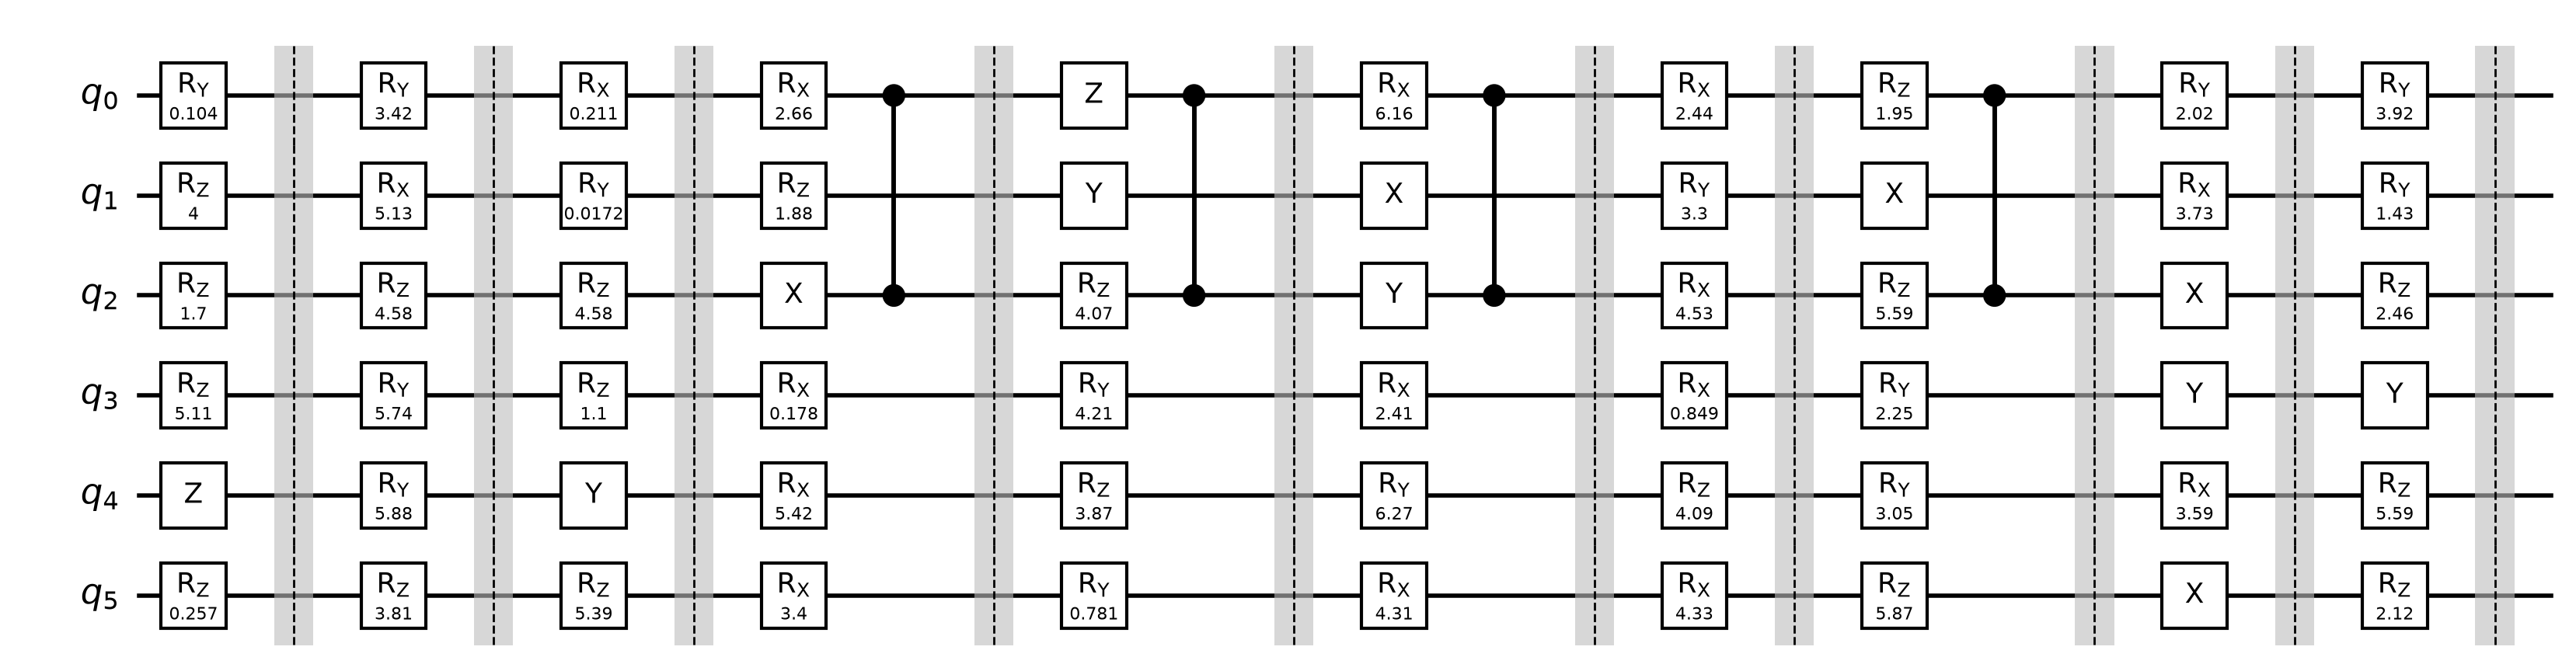
\includegraphics[width=0.95\linewidth]{figures/weak_random_example.png}
  \caption{A 6-qubit instance of the \texttt{weak\_random} benchmark
    circuit family (Section~\ref{sec:case-study:pipeline}), drawn
    directly from the pipeline's own circuit generator at a small
    qubit count for legibility. Grey dashed lines mark generation-layer
    barriers, not two-qubit gates; the only two-qubit gates present are
    four controlled-$Z$ couplings. This instance's very low
    connectivity budget allows three candidate qubit pairs
    ($q_0$--$q_2$, $q_2$--$q_3$, $q_3$--$q_4$), and this particular
    random seed's independent per-gate draw happened to pick the same
    pair, $q_0$--$q_2$, all four times.}
  \label{fig:weak-random-example}
\end{figure}

Figure~\ref{fig:interaction-graph} makes stage (1) concrete on a real
run rather than only the static circuit above: an 8-qubit
\texttt{weak\_random} instance (seed 0), partitioned by the pipeline's
current code into four blocks --
$\{0,2,4\}$, $\{1\}$, $\{3,5\}$, and $\{6,7\}$. Nodes $\{0,2,4,6,7\}$
form a single \emph{connected} component in the interaction graph --
qubit 4 bridges both halves -- yet Louvain splits it into two separate
blocks, $\{0,2,4\}$ and $\{6,7\}$, rather than only ever cutting at
already-disconnected points; qubit 1, with no interaction edges at all,
becomes its own singleton block. The edge crossed by that
$\{0,2,4\}$/$\{6,7\}$ split is exactly the kind of inter-block gate
stage (5)'s injection has to reconsider, and stage (1)'s own
partitioning choice -- not just the circuit's raw connectivity --
determines how much of that reconsideration is needed.

\begin{figure}[htbp]
  \centering
  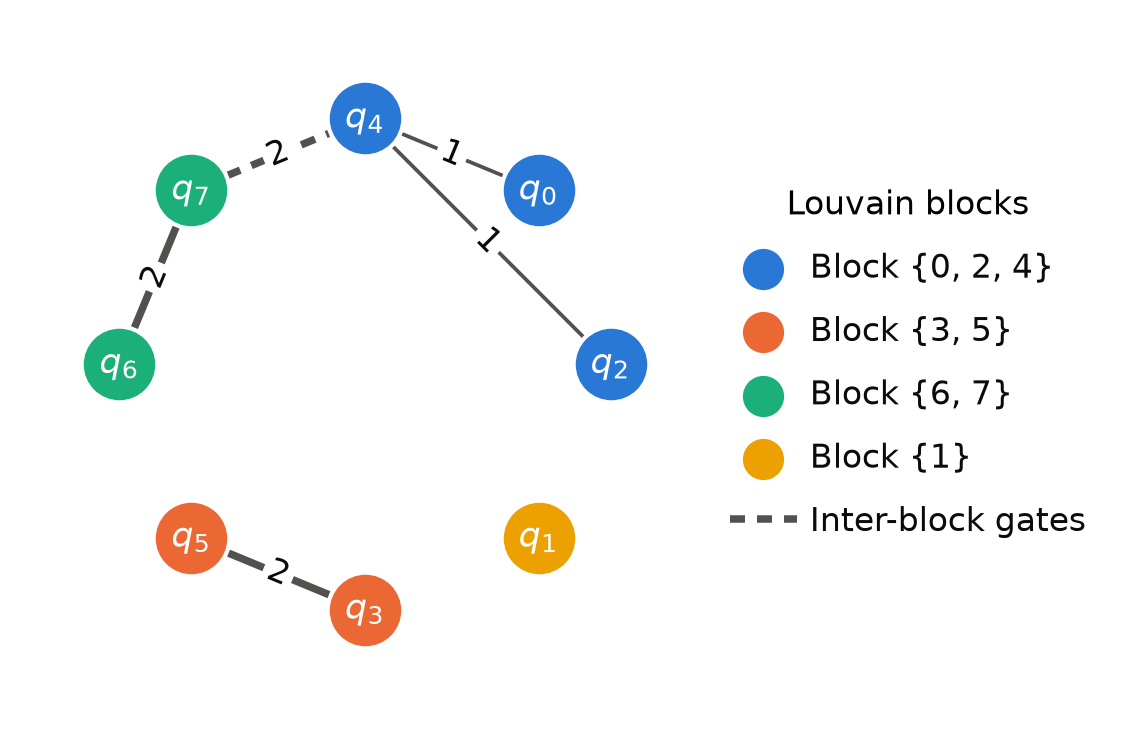
\includegraphics[width=0.75\linewidth]{figures/interaction_graph_weak_random_8q.png}
  \caption{Qubit-interaction graph for the same \texttt{weak\_random}
    family (8 qubits, seed 0, generated by running the pipeline's
    current code, not the static example above) -- edge labels are
    2-qubit gate counts, the weights Louvain community detection
    partitions on. Node colour gives each qubit's Louvain block; the
    dashed edge is the only one crossing a block boundary. Qubits are
    placed on a circle grouped by block, so position carries no
    distance meaning.}
  \label{fig:interaction-graph}
\end{figure}

\paragraph{Experimental data.}
\label{sec:case-study:data}
Every aggregate result in this section (Tables~\ref{tab:case-study-algorithms}
and~\ref{tab:case-study-hv}, Figures~\ref{fig:case-study-algorithm-fidelity}
and~\ref{fig:case-study-hv-bars})
and in Figure~\ref{fig:scaling-wallclock} is computed from a single
dataset produced for this survey: the \emph{225-run core baseline}, i.e.\
the three per-block optimizers run on the five benchmark circuit
families at each family's three qubit counts, with five random seeds
per configuration, 100 generations and a population size of 100. The
runs were completed on 6 September 2026, after the injection-stage
fix described above, on a single laptop (Intel Core i7-12700H, 64\,GB
RAM), with fitness evaluation parallelized across all CPU cores. Each
run records its configuration, per-stage wall-clock timings, final
metrics, and Pareto front; the per-run records are aggregated into one
results table, from which every figure and table is generated by
script. The pipeline code, experiment tooling, and figure-generation
scripts are available at
\url{https://github.com/gileano/code_PFE/tree/ULBS_qiea}.

\subsection{NSGA-II vs.\ SMS-EMOA vs.\ NSGA-III as a Worked Example}
\label{sec:case-study:algorithms}

The pipeline's per-block optimizer is selected through a small registry
of interchangeable functions sharing one call signature, which makes it
a concrete demonstration that the taxonomy's selection axis
(Section~\ref{sec:taxonomy:selection}) is a genuine, swappable design
dimension rather than only an abstract classification: the same
partitioning, fidelity metric, injection, and compression stages sit
around whichever of NSGA-II's crowding-distance selection, SMS-EMOA's
hypervolume-driven environmental selection, or NSGA-III's reference-point
niching is plugged in underneath. This is also, incidentally, the
reverse pairing already flagged in
Sections~\ref{sec:taxonomy:hybridization} and
\ref{sec:critical-analysis:per-category}: it demonstrates the same
three selection paradigms interchanged around one representation, but a
domain-specific, non-quantum-inspired one, not the Q-bit representation
the surveyed QIEA-MOO literature has paired with several selection
paradigms but never with reference-point or hypervolume-driven
selection.

Figure~\ref{fig:moo-evolution} shows what one such run actually looks
like under the hood, rather than only its aggregate outcome: the
hypervolume and spread of block $\{0,2,4\}$'s population, tracked every
generation, for the same \texttt{weak\_random} $n{=}8$ instance as
Figure~\ref{fig:interaction-graph}, optimized here with NSGA-II. Both
indicators move together for long stretches but neither improves
monotonically -- hypervolume repeatedly drops sharply and recovers
over the run's first two thirds, before both indicators plateau in the
final third of the run. Because NSGA-II is elitist -- the best
non-dominated individuals always survive into the next
generation -- its hypervolume measured against a \emph{fixed}
reference point and normalization should not fall, apart from small
losses when crowding-distance truncation removes points from an
over-full first front. The sharp drops in
Figure~\ref{fig:moo-evolution} are instead a measurement effect: each
generation's hypervolume is computed after normalizing the objectives
by \emph{that generation's own} population minimum and maximum, with a
reference point derived from the same bounds. Whenever a new individual
extends the population's range in some objective, the whole front
shrinks in the normalized coordinates and the hypervolume falls, even
though the front itself has not deteriorated. This is the same
per-run adaptive normalization that
Section~\ref{sec:case-study:hypervolume} shows to distort
cross-algorithm comparisons, here distorting comparisons across
generations of a single run; the curve is therefore informative about
when the population's objective ranges change, but not, on its own,
about convergence. This is the kind of
generation-by-generation behavior the aggregate
fidelity/hypervolume comparisons below necessarily average away.

\begin{figure}[htbp]
  \centering
  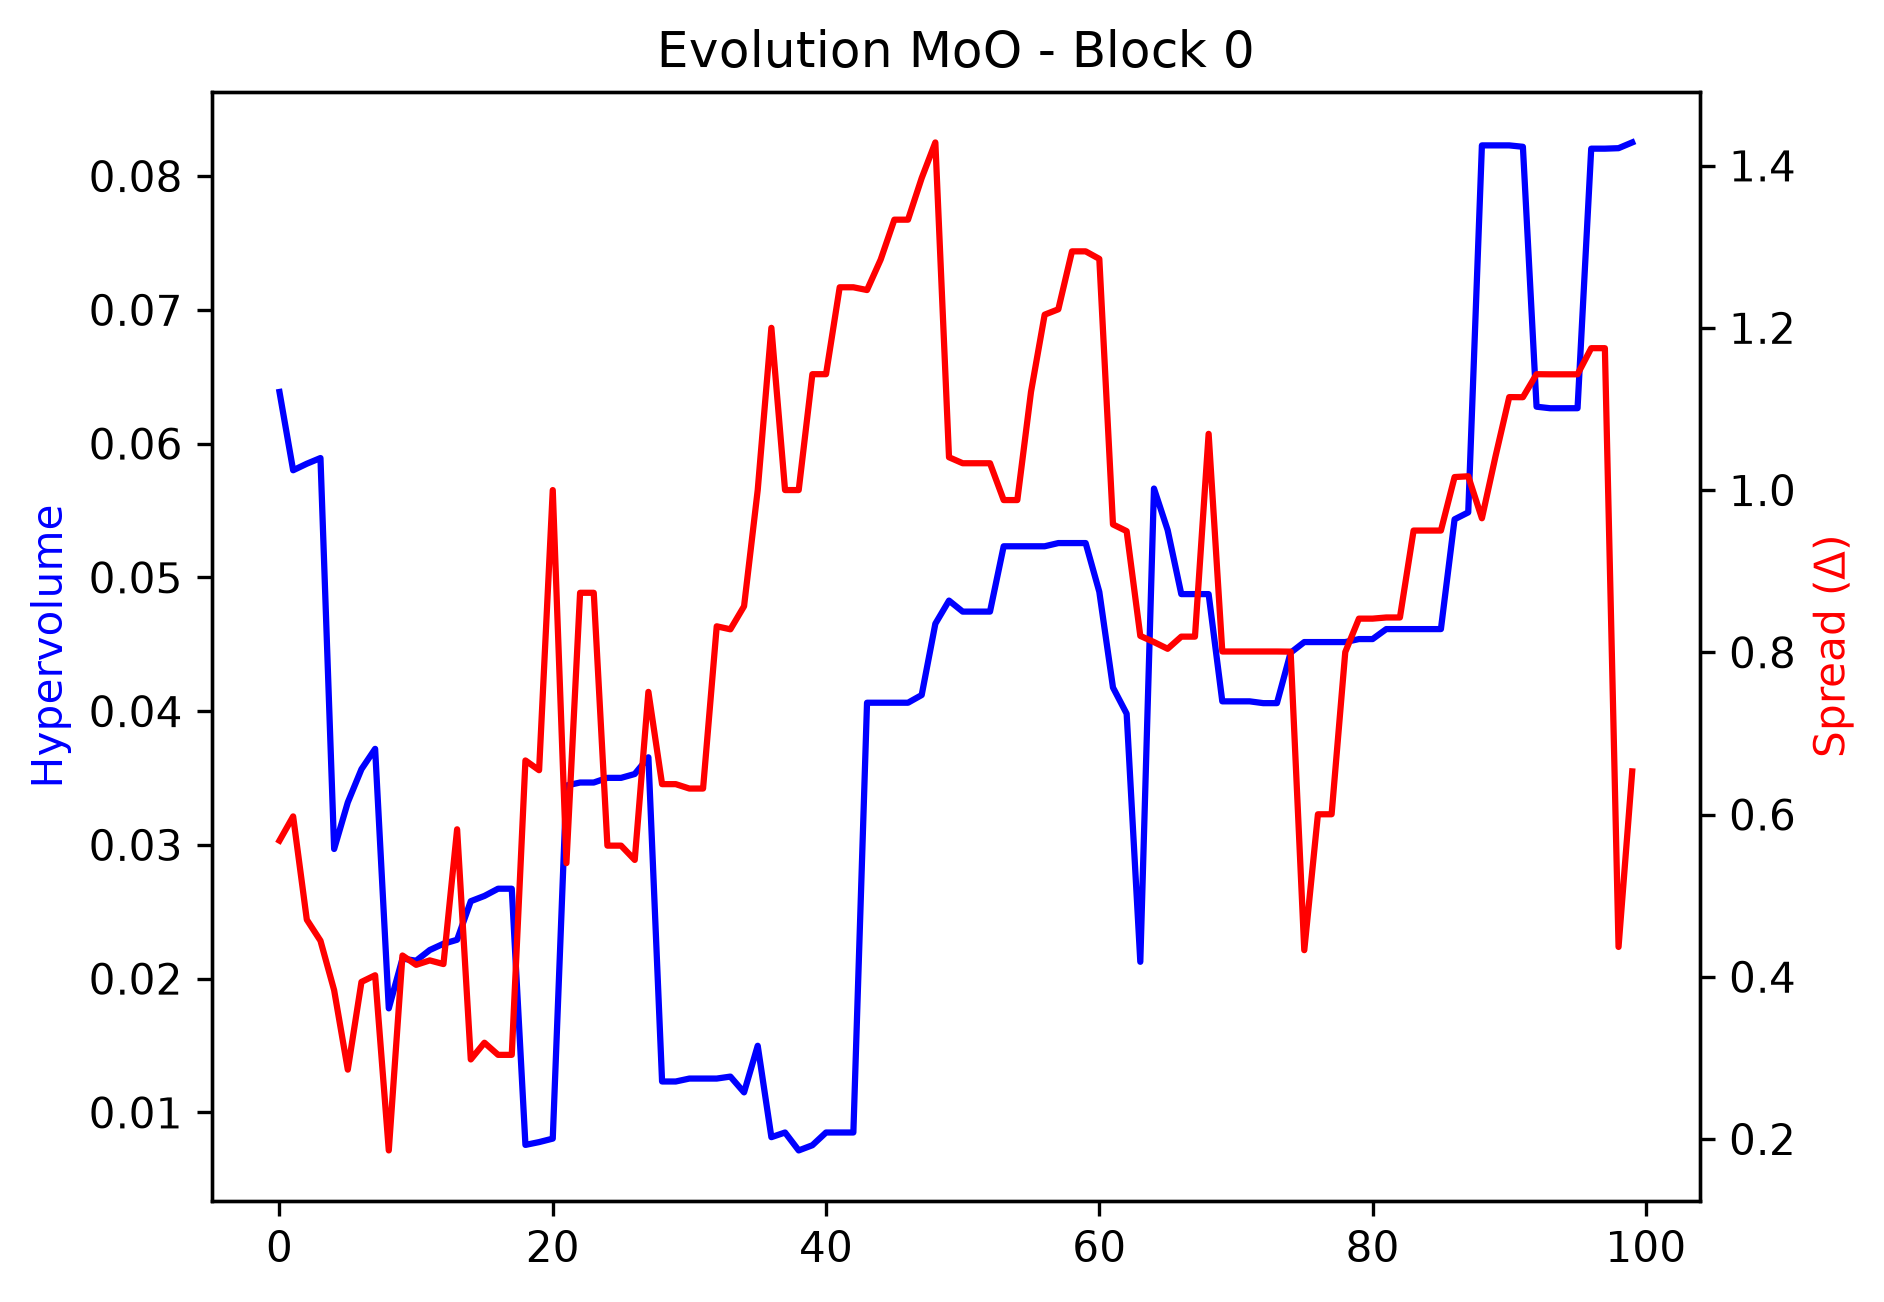
\includegraphics[width=0.85\linewidth]{figures/moo_evolution_weak_random_8q_block0.png}
  \caption{Adaptive (per-generation-normalized) hypervolume and spread
    vs.\ generation for block $\{0,2,4\}$
    of the same run as Figure~\ref{fig:interaction-graph}
    (\texttt{weak\_random}, $n{=}8$, seed 0), optimized with NSGA-II
    over 100 generations, population size 100 (the core baseline's own
    settings). Source: a single pipeline run with the core baseline's
    configuration (Section~\ref{sec:case-study:data}).}
  \label{fig:moo-evolution}
\end{figure}

Table~\ref{tab:case-study-algorithms} summarizes the 225-run core
baseline re-verified on the fixed injection-stage code (five circuit
families, each at the three qubit counts given in
Section~\ref{sec:case-study:pipeline}, three per-block optimizers, and
five seeds per configuration; point mutation, no hybrid local
search). NSGA-II reaches
the highest mean final fidelity in 13 of the 15 circuit-by-size cells;
NSGA-III wins one (\texttt{weak\_random} at $n{=}8$) and SMS-EMOA wins
one (\texttt{qft} at $n{=}12$); Figure~\ref{fig:case-study-algorithm-fidelity}
shows the pooled means. This mirrors the general shape of an
earlier, pre-fix comparison, but the two are not otherwise comparable,
since the injection-stage fix changes how much fidelity the pipeline's
later stages recover regardless of which per-block optimizer produced
the starting point. On efficiency, upstream of the injection stage and
therefore unaffected by that fix, NSGA-III's per-block optimization is
cheaper in wall-clock time than NSGA-II's in 14 of the 15 cells --
by roughly 1\% to 12\%, aggregating to about 4.5\% cheaper overall --
with a single exception (\texttt{weak\_random} at its own $n{=}20$
ceiling, where NSGA-III was about 2\% \emph{more} expensive). The
direction is consistent with the efficiency gap being caused by the
underlying evolutionary library's reference-point selection
implementation defaulting to a cheaper non-dominated-sorting routine
than the crowding-distance and hand-rolled hypervolume-driven selections
use -- an implementation detail of this pipeline's current software
stack, not a general claim that NSGA-III is more efficient than
NSGA-II as algorithms. Nor does it carry over to end-to-end cost: mean
total wall-clock per run is roughly 1.9 times \emph{higher} for NSGA-III
than for NSGA-II (331s vs.\ 176s; SMS-EMOA 124s). The whole difference
comes from two families at $n{=}20$ (\texttt{hw\_efficient\_ansatz} and
\texttt{w\_state}), and none of it from block optimization: about
two fifths falls in the injection stage and the rest outside the
pipeline's four timed stages. Why has not been established. This
distinction matters because an earlier
measurement in this same project once suggested a much larger, roughly
two-fold advantage for NSGA-III; closer, fresher re-measurement showed
that figure to be a stale-versus-fresh timing artifact rather than a
real effect, and it was retracted once the single-digit-percent figure
above was confirmed on repeated measurement. That episode is a direct,
self-inflicted instance of the single-run benchmarking weakness
Section~\ref{sec:critical-analysis:cross-cutting} raises about the wider
literature -- this project is not exempt from the risk it identifies in
others, only better positioned to catch it once measured twice.

\begin{table}[htbp]
  \centering
  \small
  \caption{Per-block-optimizer comparison on the 225-run core baseline
    (5 circuit families $\times$ 3 qubit counts $\times$ 3 optimizers
    $\times$ 5 seeds; point mutation, no hybrid local search,
    stochastic injection). ``Cells won'' counts the circuit-by-size
    cells (of 15) where that optimizer reached the highest mean
    \texttt{fidelity\_final}. Fair hypervolume is defined in
    Section~\ref{sec:case-study:hypervolume}. Source: 225-run core
    baseline (Section~\ref{sec:case-study:data}).}
  \label{tab:case-study-algorithms}
  \begin{tabularx}{\textwidth}{@{}p{2.6cm}YYYY@{}}
    \toprule
    Per-block optimizer & Mean fidelity\_final & Cells won (/15) &
    Mean block-opt.\ wall-clock (s) & Mean fair HV \\
    \midrule
    NSGA-II   & 0.110 & 13 & 42.78 & 0.808 \\
    NSGA-III  & 0.092 & 1  & 40.85 & 0.729 \\
    SMS-EMOA  & 0.092 & 1  & 43.88 & 0.788 \\
    \bottomrule
  \end{tabularx}
\end{table}

\begin{figure}[htbp]
  \centering
  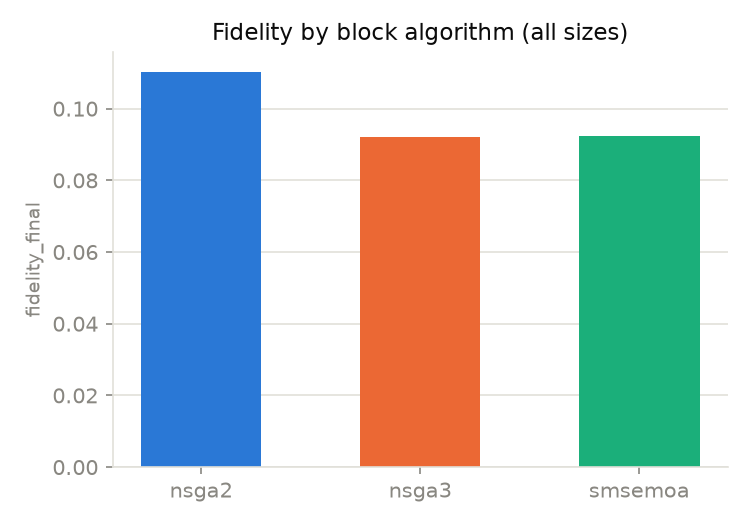
\includegraphics[width=0.6\linewidth]{figures/algorithm_fidelity.png}
  \caption{Mean \texttt{fidelity\_final} by per-block optimizer, pooled
    across all 15 circuit-by-size cells of
    Table~\ref{tab:case-study-algorithms}; each bar averages 75 runs
    (5 circuit families $\times$ 3 qubit counts $\times$ 5 seeds).
    Source: 225-run core baseline (Section~\ref{sec:case-study:data}).}
  \label{fig:case-study-algorithm-fidelity}
\end{figure}

\subsection{No Universally-Best Mutation Operator}
\label{sec:case-study:mutation}

The pipeline exposes a second, independent design axis within each
per-block optimizer: the mutation operator applied to a block's
chromosome, with point mutation (fixed-length) and two
insertion/deletion variants (variable-length) available across all
three optimizers in Section~\ref{sec:case-study:algorithms}, together
with an optional local-search refinement pass applied to the winning
individual afterward. An ablation across these mutation schemes and the
local-search option, at several problem sizes, was run and analyzed
before the injection-stage bug described in
Section~\ref{sec:case-study:pipeline} was found, and its headline
finding -- that no single mutation operator dominates uniformly across
problem scale -- has not yet been re-run on the fixed code. Because the
injection-stage bug changes how much of the final circuit's fidelity
this pipeline's later stages recover, and the local-search option's
value is entangled with exactly that recovery, that pre-fix finding
cannot be assumed to still hold and is deliberately not restated here as
a current result, pending that re-run. This is reported not as a gap in
this section so much as a demonstration of the discipline
Section~\ref{sec:critical-analysis:cross-cutting} argues the wider
QIEA-MOO literature should apply more consistently: a finding computed
on code later found to contain a real correctness bug is treated as
provisional, not citable, until it is re-derived on the corrected code,
even when -- as here -- re-running the ablation is a known, scoped, but
not yet completed piece of future work.

\subsection{Hypervolume Comparability Across Algorithms}
\label{sec:case-study:hypervolume}

A separate, purely methodological finding from this pipeline's own
quality-indicator tooling illustrates the benchmarking-practice
limitations raised in Section~\ref{sec:critical-analysis:cross-cutting}
directly, and -- unlike Section~\ref{sec:case-study:mutation}'s
ablation -- is structural rather than data-dependent, so it does not
need to wait on any re-run to be cited. The pipeline's per-run
hypervolume computation derives its reference point and normalization
adaptively from that run's own final population, which is appropriate
for tracking a single run's own convergence but not valid for ranking
different algorithms or runs against each other, since the same
absolute hypervolume value means something different depending on the
population it was normalized against. The fix is to also record each
run's Pareto front in raw, unnormalized units and, when comparing
algorithms, pool all of their front points per block into one shared
minimum/maximum normalization and one shared, fixed reference point
before computing hypervolume.

\begin{table}[htbp]
  \centering
  \small
  \caption{Adaptive (per-run-normalized) vs.\ fair (shared-reference)
    mean hypervolume, by per-block optimizer, at three scale slices of
    the 225-run core baseline. Fair HV ranks the three optimizers
    consistently across all three slices; adaptive HV does not rank
    them consistently even against itself. Source: 225-run core
    baseline (Section~\ref{sec:case-study:data}).}
  \label{tab:case-study-hv}
  \begin{tabularx}{\textwidth}{@{}p{3.4cm}YYY YYY@{}}
    \toprule
    & \multicolumn{3}{c}{Adaptive mean HV} & \multicolumn{3}{c}{Fair mean HV} \\
    \cmidrule(lr){2-4} \cmidrule(lr){5-7}
    Scale slice & NSGA-II & NSGA-III & SMS-EMOA & NSGA-II & NSGA-III & SMS-EMOA \\
    \midrule
    All 5 families, all sizes pooled & 0.048 & 0.045 & 0.055 & 0.808 & 0.729 & 0.788 \\
    All 5 families, $n{=}12$ (matched) & 0.050 & 0.045 & 0.054 & 0.812 & 0.736 & 0.808 \\
    \texttt{qaoa\_maxcut} only, its own $n{=}16$ ceiling & 0.024 & 0.030 & 0.028 & 0.810 & 0.593 & 0.739 \\
    \bottomrule
  \end{tabularx}
\end{table}

Table~\ref{tab:case-study-hv} shows both
computations, side by side, at three scale slices of the re-verified
225-run core baseline, and Figure~\ref{fig:case-study-hv-bars} plots
its pooled row. Adaptive mean HV ranks SMS-EMOA above NSGA-II
above NSGA-III when pooling all sizes, but that ranking is not even
stable against itself as the scale slice changes: at
\texttt{qaoa\_maxcut}'s own $n{=}16$ ceiling, adaptive HV instead ranks
NSGA-III above SMS-EMOA above NSGA-II -- not a strict reversal of the
pooled order (SMS-EMOA and NSGA-II swap places relative to a true
reversal), but NSGA-III still moves from worst to best.
Fair HV, by contrast, ranks NSGA-II above SMS-EMOA above NSGA-III
consistently across all three slices, and NSGA-III's fair-HV gap to
NSGA-II widens rather than narrows as problem size grows: 0.052 at
$n{=}8$ and 0.076 at $n{=}12$ (both matched across all five families),
0.084 at $n{=}20$ (the four families that reach it), and widest, 0.217,
at \texttt{qaoa\_maxcut}'s own $n{=}16$ ceiling. This is a direct, current demonstration of the risk the
adaptive-versus-fair distinction warns about: an algorithm-comparison
conclusion drawn from adaptive HV alone would not just be
questionable in the abstract, it would flip depending on which slice of
this pipeline's own data it was drawn from. The methodological point
itself, unaffected by any of these specific numbers, is what is
load-bearing: cross-algorithm hypervolume comparison requires a shared
reference point, and an adaptive, per-run one is only valid for
single-run convergence plots.

\begin{figure}[htbp]
  \centering
  \begin{minipage}{0.48\linewidth}
    \centering
    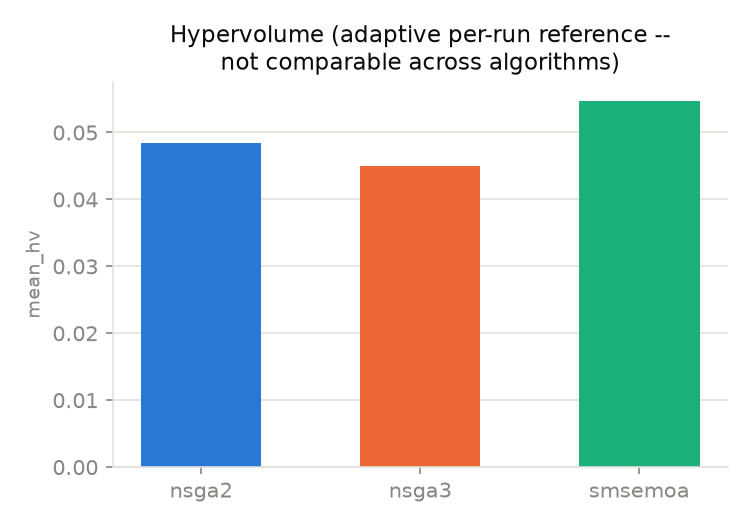
\includegraphics[width=\linewidth]{figures/algorithm_hypervolume_adaptive.png}
  \end{minipage}\hfill
  \begin{minipage}{0.48\linewidth}
    \centering
    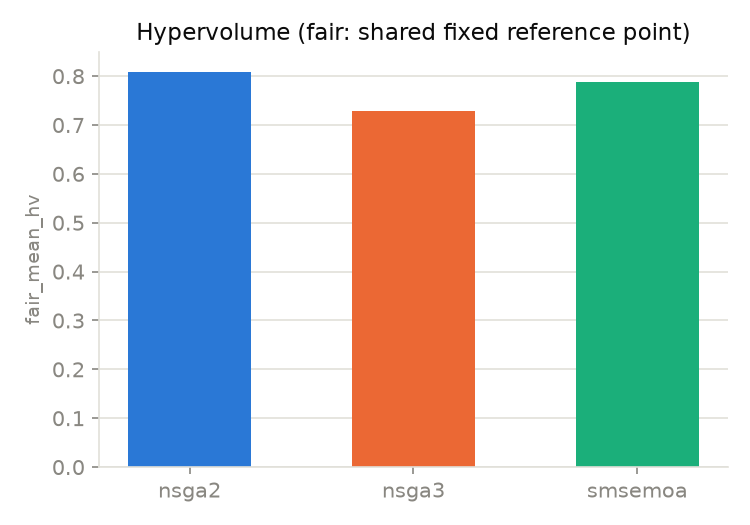
\includegraphics[width=\linewidth]{figures/algorithm_hypervolume_fair.png}
  \end{minipage}
  \caption{The pooled-all-sizes row of Table~\ref{tab:case-study-hv},
    shown visually: adaptive mean hypervolume (left, explicitly labeled
    not comparable across algorithms) ranks SMS-EMOA highest, while
    fair mean hypervolume (right) ranks NSGA-II highest and NSGA-III
    lowest -- a visibly different ranking from the same underlying
    Pareto fronts. Source: 225-run core baseline
    (Section~\ref{sec:case-study:data}).}
  \label{fig:case-study-hv-bars}
\end{figure}

A second,
purely structural guarantee from the same tooling is that the optional
local-search refinement pass mentioned in
Section~\ref{sec:case-study:mutation} cannot affect the recorded Pareto
front at all, by construction: the front is captured from the
population before that refinement runs, and the refinement only
modifies a copy of the winning individual afterward. Fair and adaptive
hypervolume are therefore always identical between local-search on and
off, at any problem size -- a claim about how the indicator is computed,
not about any experimental outcome, and one this project has not
attempted to unsettle by re-measurement because there is nothing in the
fix above that could change it. One question Table~\ref{tab:case-study-hv}
raises but does not answer -- why NSGA-III's front is not only smaller
than NSGA-II's or SMS-EMOA's under the shared-reference comparison but
increasingly so as problem size grows, a question about Deb and Jain's
reference-point niching versus crowding-distance-based and
hypervolume-driven diversity rather than about measurement artifacts --
remains open and is revisited as a candidate direction in
Section~\ref{sec:open-challenges}.

\subsection{Energy-Efficiency Implications}
\label{sec:case-study:energy}

Section~\ref{sec:introduction} motivated QIEA-for-MOO partly on
energy-efficiency grounds: reducing the resources an optimization
problem requires is part of a broader case for sustainable
computing~\citep{sai2026generative,banciu2026aiot}, and
optimization-driven resource management already delivers measurable
energy and emission savings in other domains~\citep{moga2025rlmicrogrid}.
The case study touches this argument at two distinct points, which
have to be kept apart because the evidence for each is of a different
kind: the classical compute spent \emph{running} the optimizer, and the
quantum resources the \emph{resulting} circuit would consume on
hardware. No energy was measured directly in either case; what the
225-run baseline records are compute time and circuit depth, used below
as proxies, not as energy figures.

\paragraph{Cost of the optimization itself.}
The whole baseline consumed about 13.1 hours of summed wall-clock time
on the single laptop described in Section~\ref{sec:case-study:data},
and the choice of per-block optimizer alone moves that cost
substantially: mean total wall-clock per run is 124s for SMS-EMOA,
176s for NSGA-II, and 331s for NSGA-III, a spread of about 2.7 times
between the cheapest and the most expensive optimizer on the same
circuits, sizes, and seeds. Circuit family matters at least as much,
from a mean of 48s per run for \texttt{qaoa\_maxcut} to 394s for
\texttt{hw\_efficient\_ansatz} (Table~\ref{tab:case-study-energy}),
and Figure~\ref{fig:scaling-wallclock} shows that cost growing sharply
with qubit count. The pipeline's block partitioning and Monte-Carlo
fidelity estimation are what make the 20-qubit sizes reachable on this
hardware at all, since exact fidelity computation is intractable beyond
roughly a dozen qubits (Section~\ref{sec:case-study:pipeline}). Two
caveats apply. First, compute time is a proxy for energy only under a
roughly constant power draw, which a laptop with all cores busy and
dynamic frequency scaling does not guarantee; a per-run energy
measurement would be needed before stating savings in joules. Second,
the cheapest optimizer is not the most effective one: NSGA-II, at
about 1.4 times SMS-EMOA's mean cost, reaches the highest mean
\texttt{fidelity\_final} (Table~\ref{tab:case-study-algorithms}), so an
energy-aware choice of optimizer is itself a trade-off, not a free
saving.

\paragraph{Resources of the resulting circuit.}
On quantum hardware, a shallower circuit with fewer gates means
shorter execution and less exposure to decoherence, and therefore
potentially fewer repetitions and less device time per useful result.
The optimized circuits are markedly shallower for four of the five
families -- mean depth reductions of 34\% to 66\% -- but \emph{deeper}
for \texttt{qft}, by 33\% on average
(Table~\ref{tab:case-study-energy}), so depth reduction is not
something the pipeline delivers uniformly. More importantly, depth
reductions only translate into a hardware saving if the shorter
circuit still does the same job, and on the current baseline it
mostly does not: median \texttt{fidelity\_final} across the 225 runs
is 0.029, and only two runs, both on \texttt{weak\_random}, reach a
fidelity of 0.5. A circuit that is 60\% shallower but reproduces the
target poorly is not an energy saving but a different computation.
The case study therefore supports the energy argument for the
optimization process as a measurable, controllable cost, and frames the
hardware-side saving as conditional: it becomes a claim only once the
fidelity of the shortened circuits is high enough for them to replace
the originals, which the forthcoming empirical results paper has to
establish rather than assume. The same caution applies to the
literature reviewed in Section~\ref{sec:critical-analysis}: an energy
or resource reduction reported without the quality of the solution
that achieves it is not yet evidence of efficiency.

\begin{table}[htbp]
  \centering
  \small
  \caption{Resource proxies per circuit family on the 225-run core
    baseline (45 runs per family, pooled over its three qubit counts and
    the three per-block optimizers). Depth change is relative to the
    input circuit (negative = shallower); wall-clock is per run, end to
    end. Compute time is reported, not energy. Source: 225-run core
    baseline (Section~\ref{sec:case-study:data}).}
  \label{tab:case-study-energy}
  \begin{tabularx}{\textwidth}{@{}p{3.4cm}YYYY@{}}
    \toprule
    Circuit family & Mean depth change & Mean fidelity\_final &
    Runs with fidelity $\geq 0.5$ & Mean wall-clock (s) \\
    \midrule
    \texttt{weak\_random}         & $-58\%$ & 0.321 & 2 & 105 \\
    \texttt{qaoa\_maxcut}         & $-66\%$ & 0.045 & 0 & 48 \\
    \texttt{w\_state}             & $-54\%$ & 0.057 & 0 & 334 \\
    \texttt{hw\_efficient\_ansatz} & $-34\%$ & 0.039 & 0 & 394 \\
    \texttt{qft}                  & $+33\%$ & 0.029 & 0 & 170 \\
    \bottomrule
  \end{tabularx}
\end{table}

\subsection{Hypothetical Application Scenario: Chemical Process Eco-Efficiency}
\label{sec:case-study:scenario-chemistry}

This and the next subsection apply the survey's findings to two
application domains in which energy is part of the objective itself,
not only a cost of computing: the design and operation of a chemical
production plant, and the day-ahead dispatch of an industrial
microgrid. Unlike the rest of this section, both are hypothetical. No
experiment was run for either, and no performance figure is given,
because none could be given without one. The problem formulations are
simplified for illustration and are not taken from a published study.
What the two subsections do instead is ask what the taxonomy
(Section~\ref{sec:taxonomy}) and the limitations identified in
Section~\ref{sec:critical-analysis} imply for anyone considering a
multi-objective QIEA for such a problem; Table~\ref{tab:case-study-scenarios}
summarizes the answer for both.

\paragraph{Problem.}
Consider a continuously operated plant producing methanol from syngas,
with three units:
steam methane reforming, methanol synthesis, and distillation. Three
objectives conflict: maximize net annual profit, minimize specific
greenhouse-gas emissions per tonne of methanol, and minimize specific
thermal energy consumption per tonne. The decision vector mixes
continuous operating parameters (steam-to-carbon ratio, reformer
temperature, synthesis pressure, distillation reflux ratios) with
discrete design choices (which hot and cold streams the heat-exchanger
network matches, and how many catalyst beds the synthesis reactor uses).
Evaluating one candidate requires a rigorous flowsheet simulation, so
each objective evaluation is expensive, and heat integration makes the
objective landscape discontinuous wherever the network's stream matches
change.

\paragraph{What the survey implies.}
\emph{Representation.} The decision vector sits at both ends of the
representation range of Section~\ref{sec:taxonomy:representation} at
once. The stream matches and bed count are binary or small-integer
choices, which a Q-bit chromosome observes directly; the operating
parameters are continuous and must be decoded from several Q-bits each,
which fixes their precision in advance and is the setting in which
\citet{olvera2023continuous} saw the quantum-inspired variants degrade
as the number of variables grew. None of the surveyed multi-objective
methods documents a mixed binary--continuous encoding, so the split
between the two parts of the chromosome would be the designer's own
choice. \emph{Feasibility.} Many observed stream-match combinations are
thermodynamically infeasible, and a Q-bit observation is unconstrained,
so a repair step or a penalty is unavoidable. \citet{gilea2026waste}'s
QIEA fell behind a classical genetic algorithm as its problem grew, a
loss its authors attribute to the repair step producing more and more
of each solution (Section~\ref{sec:feature-comparison}); the same risk
applies here.
\emph{Evaluation budget.} With a simulator in the loop, the number of
evaluations, not the optimizer's own overhead, sets the cost. The claim
that matters is therefore whether a QIEA reaches a given front quality
in fewer evaluations than a classical MOEA at an equal budget. The
surveyed performance claims each rest on a single problem and an
author-chosen classical baseline
(Section~\ref{sec:critical-analysis:per-category}), so they do not
establish that such an advantage would transfer to a simulator-bound
problem. \emph{Operators and selection.} The usual remedy for a
population stuck in one region of a discontinuous landscape is a
diversity-restoring operator. No surveyed multi-objective QIEA has an
interference-based or reset operator for this
(Section~\ref{sec:taxonomy:operator}); its only lever is the rotation
gate's angle schedule, so such an operator would be a contribution in
its own right, not a component to reuse. With three objectives, the
reference-point and hypervolume-driven selection that no surveyed QIEA
pairs with a Q-bit representation (Section~\ref{sec:taxonomy:selection})
would be natural candidates to try. \emph{Prior work.} A keyword
screen of the Section~\ref{sec:bibliometric} corpus found no
multi-objective QIEA for chemical process design or operation; the
closest is refinery crude-oil scheduling. A study of this scenario
would therefore be new ground for QIEA-MOO rather than a comparison
with existing work.

\subsection{Hypothetical Application Scenario: Industrial Microgrid Dispatch}
\label{sec:case-study:scenario-microgrid}

\paragraph{Problem.}
Consider a manufacturing site supplied by rooftop solar photovoltaics,
a combined heat and power (CHP) gas turbine, a battery, and a grid
connection with time-of-use tariffs and peak-demand charges. The task
is to fix the next day's dispatch schedule in 15-minute intervals, so
$T{=}96$ time steps. At each step, four quantities are decided: the
CHP unit's power output and the battery's charge or discharge power
(both continuous), whether each shiftable batch production load runs
(binary), and the heat output of an auxiliary boiler (continuous) --
$96 \times 4 = 384$ decision variables in total, with one shiftable
load. Three objectives conflict: minimize daily cost (grid energy,
fuel, and battery degradation), minimize wasted energy (CHP heat dumped
plus solar output curtailed), and minimize peak grid import. Power and
heat must balance in every interval, and the battery's state of charge
links each interval to the next.

\paragraph{What the survey implies.}
\emph{Scale.} The problem has 288 continuous variables. At an
illustrative precision of 10 Q-bits per continuous variable, the
chromosome would hold 2,976 Q-bits, far beyond the problems on which
\citet{olvera2023continuous} already saw performance degrade with the
number of decision variables. \emph{Coupling across time.} Each Q-bit
is observed independently, so the representation itself carries no
dependency between genes: a schedule observed from a Q-bit chromosome
can drain the battery at one interval and need it two hours later. The
state-of-charge constraint has to be enforced by repair or penalty, with
the same scaling risk as in the chemical scenario. The only
entanglement-inspired operator in the surveyed set, the crossover of
\citet{kumar2026eahqnsga2}, couples pairs of individuals
(Section~\ref{sec:taxonomy:operator}), not genes within one chromosome,
so no surveyed operator addresses this kind of dependency. \emph{Run time.} A dispatch
schedule recomputed every 15 minutes, as in model-predictive control,
must be produced within that interval. The case study shows that the
choice of optimizer alone moved compute cost by a factor of about 2.7
(Section~\ref{sec:case-study:energy}), and \citet{gilea2026waste}'s
QIEA took about 3.85 times a classical genetic algorithm's running time,
so wall-clock time would have to be reported next to front quality,
not inferred from the number of generations. \emph{Prior work.} Unlike
the chemical scenario, this domain is not new to quantum-inspired
optimization. The most-cited power-system QIEA in the corpus solves
dynamic economic dispatch with wind generation as a single-objective
problem~\citep{lee2011qgadispatch}, and the corpus also contains
multi-objective QIEAs for economic--emission dispatch and microgrid
capacity allocation, outside the in-depth set of
Section~\ref{sec:critical-analysis}. Reinforcement learning is an
established alternative for microgrid energy
management~\citep{moga2025rlmicrogrid}. A QIEA-MOO study of this
scenario would therefore need to compare against these existing
methods, and against each other, which is the comparison
Section~\ref{sec:critical-analysis:per-category} found missing.
\emph{Reporting.} The lesson of Section~\ref{sec:case-study:energy}
applies directly: an energy saving such as less dumped heat counts only
alongside the cost and peak-import values of the same schedule, and
fronts from different optimizers have to be compared with a shared
hypervolume reference point (Section~\ref{sec:case-study:hypervolume}).

\begin{table}[htbp]
  \centering
  \small
  \caption{The two hypothetical application scenarios of
    Sections~\ref{sec:case-study:scenario-chemistry}
    and~\ref{sec:case-study:scenario-microgrid}, read against the
    survey's taxonomy and limitations. Both formulations are
    illustrative; no experiment was run and no result is reported.}
  \label{tab:case-study-scenarios}
  \begin{adjustwidth}{-2cm}{-2cm}
  \centering
  \begin{tabularx}{\linewidth}{@{}>{\raggedright\arraybackslash}p{2.9cm}YY@{}}
    \toprule
    & Chemical plant (methanol) & Industrial microgrid \\
    \midrule
    Objectives & Profit; specific emissions; specific thermal energy &
      Daily cost; wasted energy; peak grid import \\
    Decision variables & Mixed: continuous operating parameters, discrete
      heat-exchanger matches and bed count &
      384: 288 continuous, 96 binary (96 steps $\times$ 4) \\
    Representation issue & Mixed binary--continuous encoding, not
      documented by any surveyed method &
      Thousands of Q-bits after decoding; no inter-gene dependency \\
    Feasibility & Infeasible stream matches; repair or penalty &
      Power/heat balance, battery state of charge linking intervals \\
    Dominant cost & Simulator calls (equal-budget comparison needed) &
      Wall-clock within a 15-minute control interval \\
    Operator gap & No diversity-restoring (interference or reset)
      operator in MO QIEAs & No operator couples genes within a
      chromosome \\
    Prior QIEA work & None found in the corpus &
      Single- and multi-objective dispatch QIEAs exist \\
    \bottomrule
  \end{tabularx}
  \end{adjustwidth}
\end{table}

Both scenarios have the features on which the surveyed literature gives
the least guidance: mixed or very many decision variables, hard
constraints, evaluations that are expensive or must finish within a
fixed time, and three objectives. That makes them candidate benchmarks
for the open questions of Section~\ref{sec:open-challenges} rather than
demonstrations that QIEA-MOO suits them. Whether it does is an
empirical question, which is precisely why no answer is given here.
